\documentclass[11pt, oneside]{article}   	% use "amsart" instead of "article" for AMSLaTeX format
\usepackage{geometry}                		% See geometry.pdf to learn the layout options. There are lots.
\geometry{letterpaper}                   		% ... or a4paper or a5paper or ... 
%\geometry{landscape}                		% Activate for for rotated page geometry
%\usepackage[parfill]{parskip}    		% Activate to begin paragraphs with an empty line rather than an indent
\usepackage{graphicx}				% Use pdf, png, jpg, or eps§ with pdflatex; use eps in DVI mode
								% TeX will automatically convert eps --> pdf in pdflatex		
\usepackage{amssymb}
\usepackage{amsmath}
\usepackage{float}
\usepackage{mathbbol}
\usepackage{algorithm, algpseudocode}

\title{A Brief Review on Biological Growth}
\author{Jie Cheng}
%\date{}							% Activate to display a given date or no date

\begin{document}
\maketitle

% new commands for the CHT paper defined by Fanlong are listed at the very bottom

\renewcommand{\url}[1]{}% ******** Remove URL's from bibtex entries ********
\newcommand{\citeCount}[1]{}% for citation counts papers for WDH citations
% 
\newtheorem{theorem}{Theorem}
\newtheorem{Algorithm}{Algorithm}
\newtheorem{procedure}{Procedure}
\newtheorem{lemma}{Lemma}
\newtheorem{definition}{Definition}
\newtheorem{proposition}{Proposition}
\newtheorem{assumption}{Assumption}
\newtheorem{condition}{Condition}
% \newtheorem{AMPInterfaceCondition}{AMP Interface Condition}
\newtheorem{AMPInterfaceCondition}{Interface Condition}
\newtheorem{modelProblem}{Model Problem}
\newtheorem{travelingWave}{Traveling Wave Exact Solution}

\newtheorem*{algorithmAMP}{AMP Algorithm (added-mass partitioned) }
\newtheorem*{algorithmTP}{TP Algorithm (traditional partitioned)}

\newtheorem*{ModelProblemIA}{Model Problem MP-IA}
\newtheorem*{ModelProblemVA}{Model Problem MP-VA}
\newtheorem*{ModelProblemVE}{Model Problem MP-VE}

\newcommand{\dx}{\Delta x}
\newcommand{\dy}{\Delta y}
\newcommand{\dt}{\Delta t}


% \newcommand{\kappaR}{{\rhoR\cR^2}}

\newcommand{\Dp}{D_{+}}
\newcommand{\Dm}{D_{-}}
\newcommand{\Dpx}{D_{+x}}
\newcommand{\Dmx}{D_{-x}}
\newcommand{\Dpy}{D_{+y}}
\newcommand{\Dmy}{D_{-y}}

\newcommand{\erf}{\operatorname{erf}}

    
\newcommand{\bogus}[1]{{}}

% -----Bill's common definitions-----

\newcommand{\av}{\mathbf{ a}}
\newcommand{\bv}{\mathbf{ b}}
\newcommand{\cv}{\mathbf{ c}}
\newcommand{\dv}{\mathbf{ d}}
\newcommand{\ev}{\mathbf{ e}}
\newcommand{\fv}{\mathbf{ f}}
\newcommand{\gv}{\mathbf{ g}}
\newcommand{\hv}{\mathbf{ h}}
\newcommand{\iv}{\mathbf{ i}}
\newcommand{\jv}{\mathbf{ j}}
\newcommand{\kv}{\mathbf{ k}}
\newcommand{\lv}{\mathbf{ l}}
\newcommand{\mv}{\mathbf{ m}}
\newcommand{\nv}{\mathbf{ n}}
\newcommand{\ov}{\mathbf{ o}}
\newcommand{\pv}{\mathbf{ p}}
\newcommand{\qv}{\mathbf{ q}}
\newcommand{\rv}{\mathbf{ r}}
\newcommand{\sv}{\mathbf{ s}}
\newcommand{\tv}{\mathbf{ t}}
\newcommand{\uv}{\mathbf{ u}}
\newcommand{\vv}{\mathbf{ v}}
\newcommand{\wv}{\mathbf{ w}}
\newcommand{\xv}{\mathbf{ x}}
\newcommand{\yv}{\mathbf{ y}}
\newcommand{\zv}{\mathbf{ z}}
% 
\newcommand{\Av}{\mathbf{ A}}
\newcommand{\Bv}{\mathbf{ B}}
\newcommand{\Cv}{\mathbf{ C}}
\newcommand{\Dv}{\mathbf{ D}}
\newcommand{\Ev}{\mathbf{ E}}
\newcommand{\Fv}{\mathbf{ F}}
\newcommand{\Gv}{\mathbf{ G}}
\newcommand{\Hv}{\mathbf{ H}}
\newcommand{\Iv}{\mathbf{ I}}
\newcommand{\Jv}{\mathbf{ J}}
\newcommand{\Kv}{\mathbf{ K}}
\newcommand{\Lv}{\mathbf{ L}}
\newcommand{\Mv}{\mathbf{ M}}
\newcommand{\Nv}{\mathbf{ N}}
\newcommand{\Ov}{\mathbf{ O}}
\newcommand{\Pv}{\mathbf{ P}}
\newcommand{\Qv}{\mathbf{ Q}}
\newcommand{\Rv}{\mathbf{ R}}
\newcommand{\Sv}{\mathbf{ S}}
\newcommand{\Tv}{\mathbf{ T}}
\newcommand{\Uv}{\mathbf{ U}}
\newcommand{\Vv}{\mathbf{ V}}
\newcommand{\Wv}{\mathbf{ W}}
\newcommand{\Xv}{\mathbf{ X}}
\newcommand{\Yv}{\mathbf{ Y}}
\newcommand{\Zv}{\mathbf{ Z}}

\newcommand{\collon}{:}  % note \colon already defined by someone.
\newcommand{\ff}{\tt}

% \newcommand{\lt}{{<}}
% \newcommand{\grad}{\nabla}
% \newcommand{\comma}{~~~,~~}
% \newcommand{\calo}{{\cal O}}

\newcommand{\half}{{1\over2}}

\newcommand{\Real}{{\mathbb R}}
\newcommand{\Complex}{{\mathbb C}}

\newcommand{\zerov}{\mathbf{0}}


\newcommand{\Ac}{{\mathcal A}}
\newcommand{\Bc}{{\mathcal B}}
\newcommand{\Cc}{{\mathcal C}}
\newcommand{\Dc}{{\mathcal D}}
\newcommand{\Ec}{{\mathcal E}}
\newcommand{\Gs}{{\mathcal G}}
\newcommand{\Ic}{{\mathcal I}}
\newcommand{\Rc}{{\mathcal R}}
\newcommand{\Gc}{{\mathcal G}}
\newcommand{\Lc}{{\mathcal L}}
\newcommand{\Nc}{{\mathcal N}}
\newcommand{\Oc}{{\mathcal O}}
\newcommand{\Pc}{{\mathcal P}}
\newcommand{\Qc}{{\mathcal Q}}
\newcommand{\Tc}{{\mathcal T}}



\newcommand{\deltav}{\boldsymbol{\delta}}
\newcommand{\omegav}{\boldsymbol{\omega}}
\newcommand{\tauv}{\boldsymbol{\tau}}
\newcommand{\phiv}{\boldsymbol{\phi}}
\newcommand{\psiv}{\boldsymbol{\psi}}
\newcommand{\sigmav}{\boldsymbol{\sigma}}
\newcommand{\chiv}{\boldsymbol{\chi}}


\newcommand{\grad}{\nabla}

% \newcommand{\tableFont}{\scriptsize}
\newcommand{\tableFont}{\footnotesize}
\newcommand{\tableFontSize}{\tableFont}
\newcommand{\num}[2]{#1e#2} % Use this macro to define the format of the numbers in the table
\newcommand{\errFormat}[1]{$e_{#1}$} % form of error label in tables
\newcommand{\eem}{e^{(j)}}
\newcommand{\rateLabel}{rate}

\clearpage
\newcommand{\dtau}{\delta_\tau}
\newcommand{\Gb}{G}


\newcommand{\As}{\bar{A}}
\newcommand{\Ks}{\bar{K}}
% \newcommand{\Fs}{\bar{F}}

\newcommand{\rhos}{\bar{\rho}}
\newcommand{\cp}{\bar{c}_p}
\newcommand{\cs}{\bar{c}_s}
\newcommand{\kappas}{{\rhos\cs^2}}
\newcommand{\zs}{{\bar {z}}}  % solid impedance based on c_p
\newcommand{\zp}{z_p}  % solid impedance based on c_s
\newcommand{\us}{\bar{u}}
\newcommand{\qs}{\bar{q}}
\newcommand{\vs}{\bar{v}}
\newcommand{\sigmas}{\bar{\sigma}}
\newcommand{\xs}{\bar{x}}
\newcommand{\xsv}{\bar{\xv}}
\newcommand{\gsv}{\bar{\gv}}
\newcommand{\rsv}{\bar{\rv}}
\newcommand{\rs}{\bar{r}}
\newcommand{\xf}{{x}}
\newcommand{\dxs}{\Delta{\bar x}}
\newcommand{\dxf}{{\Delta x}}
\newcommand{\Ns}{\bar{N}}
\newcommand{\Nf}{{N}}
\newcommand{\zf}{z_f}

\newcommand{\usv}{\bar{\uv}}
\newcommand{\vsv}{\bar{\vv}}
\newcommand{\wsv}{\bar{\wv}}

\newcommand{\ush}{\hat{\us}}
\newcommand{\usvh}{\hat{\usv}}
\newcommand{\vvh}{\hat{\vv}}
\newcommand{\vh}{\hat{v}}
\newcommand{\ph}{\hat{p}}

\newcommand{\nsv}{\bar{\nv}}
\newcommand{\vvs}{\bar{\vv}}
\newcommand{\uvs}{\bar{\uv}}
\newcommand{\xvs}{\bar{\xv}}
\newcommand{\sigmavs}{\bar{\sigmav}}
\newcommand{\sigmasv}{\bar{\sigmav}}
\newcommand{\fsv}{\bar{\fv}}
\newcommand{\qsv}{\bar{\qv}}

\newcommand{\qsvp}{\qsv^p}
\newcommand{\qsvI}{\qsv^I}
\newcommand{\qvI}{\qv^I}

\newcommand{\vvI}{\vv^I}
\newcommand{\tauvI}{\tauv^I}
\newcommand{\vvIf}{\vv^f}
\newcommand{\tauvIf}{\tauv^f}
% \newcommand{\vvIf}{\vv^{I,f}}
\newcommand{\sigmavI}{\sigmav^I}
\newcommand{\vsvIs}{\vsv^s}
\newcommand{\sigmavIs}{\sigmav^s}

\newcommand{\dvel}{{\delta_v}}
\newcommand{\vDot}{\dot{v}}
\newcommand{\vsDot}{\dot{\vs}}
\newcommand{\vvDot}{\dot{\vv}}
\newcommand{\vsvDot}{\dot{\vsv}}

% \newcommand{\rb}{r_b} % a point on the body surface

% \newcommand{\amp}{{\mathcal{A}}}
\newcommand{\amp}{A}


% \newcommand{\Energy}{\mathcal{E}}% Energy of the fluid
% \newcommand{\Area}{\mathcal{A}_b}
% \newcommand{\Area}{A_b}
% \newcommand{\width}{\mathcal{W}}
% \newcommand{\width}{w_b}


\newcommand{\charSpeed}{s}% Char. speed
\newcommand{\charVar}{\chi}% Char. variable


\newcommand{\largess}{\sffamily\large}
\newcommand{\Largess}{\sffamily\Large}
\newcommand{\bfss}{\sffamily\bfseries}
\newcommand{\smallss}{\sffamily\small}
\newcommand{\normalss}{\sffamily}
\newcommand{\scriptsizess}{\sffamily\scriptsize}

\newcommand{\hs}{\bar{h}}
% \newcommand{\Hs}{H_s}
\newcommand{\Hs}{\bar{H}}

\newcommand{\kxHat}{\hat{k}_x}
\newcommand{\kyHat}{\hat{k}_y}
\newcommand{\omegaHat}{\hat{\omega}}
\newcommand{\aHat}{\hat{a}}
\newcommand{\bHat}{\hat{b}}

\newcommand{\aTilde}{\tilde{a}}
\newcommand{\bTilde}{\tilde{b}}

\newcommand{\qsHat}{\hat{\qs}}
\newcommand{\phase}{x_0}
\newcommand{\phaset}{t_0}

\newcommand{\as}{\bar{a}}
\newcommand{\bs}{\bar{b}}
\newcommand{\ds}{\bar{d}}
\newcommand{\asHat}{\hat{\as}}
\newcommand{\bsHat}{\hat{\bs}}
\newcommand{\dsHat}{\hat{\ds}}

\newcommand{\dHat}{\hat{d}}
\newcommand{\pHat}{\hat{p}}
\newcommand{\qHat}{\hat{q}}
\newcommand{\vHat}{\hat{v}}
\newcommand{\vvHat}{\hat{\vv}}
\newcommand{\vsHat}{\hat{\vs}}
\newcommand{\sigmaHat}{\hat{\sigma}}
\newcommand{\sigmasHat}{\hat{\sigmas}}

\newcommand{\lambdas}{\bar{\lambda}}% solid Lame' parameter
\newcommand{\mus}{\bar{\mu}}% solid Lame' parameter

\newcommand{\OmegaF}{\Omega^F}% fluid domain
\newcommand{\OmegaS}{\Omega^S}% solid domain

\newcommand{\OmegaFh}{\Omega^F_h}% fluid domain
\newcommand{\OmegaSh}{\Omega^S_h}% solid domain

\newcommand{\GammaI}{\Gamma}% Fluid-Solid Interface
\newcommand{\Gammas}{\bar{\Gamma}}% Fluid-Solid Interface, reference space
\newcommand{\GammaIh}{\Gamma_h}% Fluid-Solid Interface

\renewcommand{\zp}{\bar{z}_p}
\renewcommand{\zs}{\bar{z}_s}
\newcommand{\zb}{\bar{z}}
\newcommand{\Lt}{\tilde{L}}

\newcommand{\MR}{M_r}% added mass ratio
\newcommand{\Mr}{\mathcal{M}}% another added mass ratio

\newcommand{\phis}{\phi_s}
\newcommand{\phib}{\phi_b}
% \newcommand{\phit}{\tilde{\phi}}
% \newcommand{\phit}{\phi_<}

\newcommand{\phim}{\phi_-}
\newcommand{\phip}{\phi_+}


\newcommand{\lambday}{\lambda}% 
\newcommand{\lambdax}{\lambda_x}% 

\newcommand{\cb}{\bar{c}}
\newcommand{\kk}{k_x} % wave number of 2d analysis
\newcommand{\kx}{k_x} % wave number of 2d analysis
\newcommand{\ax}{\alpha \amp^{m+1}}
\newcommand{\thetaj}{\theta} % Jeff's theta


% Predicted states:
% \newcommand{\vvp}{\vv^p}
% \newcommand{\vp}{v^p}
\newcommand{\sigmavp}{\sigmav^p}
\newcommand{\sigmap}{\sigma^p}
\newcommand{\tauvp}{\tauv^p}
\newcommand{\taup}{\tau^p}
\newcommand{\vsvp}{\vsv^p}
\newcommand{\vsp}{\vs^p}
\newcommand{\sigmasvp}{\sigmasv^p}
\newcommand{\sigmasp}{\sigmas^p}


\newcommand{\Ck}{C_k}
\newcommand{\Sk}{S_k}
\newcommand{\Ca}{C_\alpha}
\newcommand{\Sa}{S_\alpha}

\newcommand{\Sas}{S_a}
\newcommand{\Cas}{C_a}
\newcommand{\Sbs}{S_b}
\newcommand{\Cbs}{C_b}

\newcommand{\dsf}{\delta}


\newcommand{\expkw}{e^{i(k x -\omega t)}}
% \newcommand{\ampe}{\Ac_0}% amplitude of exact solution
\newcommand{\ampe}{{\bar u_{{\rm max}}}}


% \newcommand{\nus}{\bar\nu}
\newcommand{\betas}{\bar\beta}
% \newcommand{\ly}{\ell_y}
% \newcommand{\lx}{\ell_x}
% \newcommand{\ly}{\beta_y}
% \newcommand{\lx}{\beta_x}
% \newcommand{\ly}{\alpha_y}
% \newcommand{\lx}{\alpha_x}
\newcommand{\ly}{\lambda_y}
\newcommand{\lx}{\lambda_x}
% \newcommand{\ly}{\gamma_y}
% \newcommand{\lx}{\gamma_x}

\newcommand{\tanv}{\tv}% tangent 
\newcommand{\blue}{\color{blue}}
\newcommand{\red}{\color{red}}
\newcommand{\green}{\color{green}}

\newcommand{\strutt}{\rule{0pt}{10pt}}% strutt to make table height bigger
\newcommand{\tr}{\text{tr}}% trace


\newcommand{\nd}{{n_d}} % number of space dims


% JCP \newcommand{\Fig}{Fig.} % refer to figures this way
\newcommand{\Fig}{Figure} % refer to figures this way
\newcommand{\wvs}{\bar{\wv}}% solid `w
% \newcommand{\wsv}{\bar{\wv}}% solid `w

% \newcommand{\as}{c_p}% solid compression wave speed 
% \newcommand{\azs}{c_p}% solid compression wave speed 

\newcommand{\Pbar}{\bar{P}}
\newcommand{\Fbar}{\bar{F}}
\newcommand{\Ps}{\Pbar}
\newcommand{\Fs}{\Fbar}
% \newcommand{\fs}{{\bar{f}}


% \newcommand\Omegaf{{\Omega}}
\newcommand\Omegas{{\bar\Omega}}
% \newcommand\Gammas{{\bar\Gamma}}
% \newcommand\ps{{\bar P}}
% \newcommand\ks{{\bar K}}
% \newcommand\js{{\bar J}}
% \newcommand\Ss{{\bar S}}
% \newcommand\es{{\bar E}}
% \newcommand\Cs{{\tilde E}}
% \newcommand\CC{{\bar C}}
% \newcommand\stressStrain{{\cal S}}
% 
% \newcommand{\Js}{\bar{J}}


\newcommand\Ts{{\bar T}}
%\newcommand\tsv{{\bar\tv}}
\newcommand\ns{{\bar n}}
\newcommand\ts{{\bar\tau}}
%\newcommand\ts{{\bar t}}
% \newcommand\leftv{{\bar\yv}}
% \newcommand\vvr{{\tilde\vv}}
% \newcommand\rotation{{R}}
% \newcommand\leftvr{{\tilde\yv}}
% \newcommand\vr{{\tilde v}}

%\newcommand\stress{{\bar s}}
%\newcommand\stressv{{\bar\sv}}
%\newcommand\stressvr{{\tilde\sv}}
%\newcommand\stressfv{{\sv}}
%\newcommand\stressf{{s}}
%\newcommand\stressr{{\tilde s}}
\newcommand\stress{{\bar w}}
\newcommand\stressv{{\bar\wv}}
\newcommand\stressvr{{\tilde\wv}}
\newcommand\stressfv{{\wv}}
\newcommand\stressf{{w}}
\newcommand\stressr{{\tilde w}}


% -- prime variables
\newcommand{\xp}{x'}
\newcommand{\vp}{v'}
\newcommand{\xsp}{\xs'}
\newcommand{\Pp}{P'}
\newcommand{\Tp}{T'}
\newcommand{\qvp}{\qv'}
\newcommand{\qpv}{\qvp}

% interface point:
\newcommand\Qs{{\bar Q}}
\newcommand\Qf{{Q}}
\newcommand{\interfacePoint}{\Qf}
\newcommand{\interfacePointSolid}{\Qs}% in solid ref frame

\newcommand{\Gep}{\Gc_{ep}} % elastic piston grid
\newcommand{\Gd}{\Gc_{\text{rd}}}% rotating disk grid
\newcommand{\Ge}{\Gc_{e}} % deforming ellipse

\newcommand\ths{{\bar\theta}}
\newcommand\usr{{\us_r}}
\newcommand\ust{{\us_\theta}}
\newcommand\psr{{\tilde P}}
\newcommand\Vr{{\bar V}}

\newcommand\Jg{J_g}
\newcommand\Jsg{\Js_g}

\newcommand{\timeScale}{t^*}

% tangent: 
\newcommand\tn{{t}}
\newcommand\tnv{{\mathbf{t}}}
\newcommand\tns{{\bar\tn}}
\newcommand\tnvs{{\bar\tnv}}
\renewcommand\tv{\tnv}
\newcommand\tsv{\tnvs}


\newcommand\bsolid{{\bar b}}

\newcommand{\shift}{E}% shift operator


% \newcommand{\omegav}{\boldsymbol{\omega}}
\newcommand{\cm}{{\rm cm}}
\newcommand{\mrb}{m_{b}}% mass of the body
% \newcommand{\xvcm}{\xv_{\rm cm}}% position of the center of mass
% \newcommand{\vvcm}{\vv_{\rm cm}}% velocity of the center of mass
% \newcommand{\avcm}{\av_{\rm cm}}% acceleration of the center of mass
% \newcommand{\dotxvcm}{\dot\xv_{\rm cm}}% position of the center of mass
% \newcommand{\dotvvcm}{\dot\vv_{\rm cm}}% velocity of the center of mass
\newcommand{\xcm}{x_b}% position of the center of mass
\newcommand{\vcm}{v_b}% position of the center of mass
\newcommand{\xb}{x_b}% position of the center of mass
\newcommand{\vb}{v_b}% position of the center of mass
\newcommand{\xvb}{\xv_b}% position of the center of mass
\newcommand{\vvb}{\vv_b}% position of the center of mass
\newcommand{\avb}{\av_b}% acceleration of the center of mass
\newcommand{\bvb}{\bv_b}% angular acceleration of the center of mass
\newcommand{\xvcm}{\xv_b}% position of the center of mass
\newcommand{\vvcm}{\vv_b}% velocity of the center of mass
\newcommand{\avcm}{\av_b}% acceleration of the center of mass
\newcommand{\dotxcm}{\dot{x}_b}% position of the center of mass
\newcommand{\dotrb}{\dot{r}_b}% position of the center of mass
\newcommand{\dotvcm}{\dot{v}_b}% position of the center of mass
\newcommand{\dotvb}{\dot{v}_b}% position of the center of mass
\newcommand{\dotxvcm}{\dot\xv_b}% position of the center of mass
\newcommand{\dotvvcm}{\dot\vv_b}% velocity of the center of mass


% \newcommand{\dtau}{\delta_\tau}
% \newcommand{\Gb}{G}

\newcommand{\OmegaMatrix}{W}
\newcommand{\Force}{\mathcal{F}}
\newcommand{\Forcev}{\boldsymbol{\Force}}
\newcommand{\Forcevtilde}{\widetilde{\Forcev}}
\newcommand{\Fvtilde}{\Forcevtilde}
\newcommand{\Torque}{\mathcal{T}}
\newcommand{\Torquev}{\boldsymbol{\Torque}}
\newcommand{\Torquevtilde}{\widetilde{\Torquev}}
\newcommand{\Gvtilde}{\Torquevtilde}
\newcommand{\Ma}{A_m}

\newcommand{\mass}{{m_b}}
\newcommand{\force}{\Force}

%Fanlong's new commands
\newcommand{\f}{\frac}
\newcommand{\p}{\partial}
\newcommand{\ka}{\kappa}
\newcommand{\Kc}{{\mathcal K}}
\newcommand{\Tb}{{\bar T}}
\newcommand{\Ub}{{\bar U}}
\newcommand{\Kb}{{\bar {\mathcal K}}}
\newcommand{\Db}{{\bar {\mathcal D}}}

\section{Introduction}
Hyperelastic models have been successfully applied to various types of biomaterial scaling from onion epidermis \cite{Qian} to breast tissues \cite{OHagen}, from carotid vessels \cite{Zidi, Zidi2, Bols} to breast tumors \cite{Oberai}, and a number of animal organs including brain \cite{Karimi, Samani, Gilchrist}, lung  \cite{Wall, Wall2}, liver and kidney \cite{Fu, Untaroiu, Willinger}. A detailed review of the applications of isotropic hyperelastic models on biological tissues is provided in \cite{Kupriyanova}.
According to \cite{Steinmann}, hyperelastic models can be classified as phenomenological or micro-mechanical. The latter are derived from statistical mechanics arguments on networks of idealized chain molecules while the former utilize more or less complex, frequently polynomial formulations in terms of strain invariants or principle stretches. Because of the popularity of hyperelastic models, many commercial software have hyperelastic models as a built-in material selection. For instance, Abaqus FEA offers Mooney-Rivlin model, Yeoh model, neo-Hookean model, etc. It also allows the user to provide a subroutine to define new models. But there are certain limitations with commercial software. One of them is that it is not allowed to model a completely incompressible material for the purpose of the robustness of the computation \cite{Abaqus}. However, as we will demonstrate in this work, with some simple modifications complete incompressibility in finite element method can be easily achieved based on nearly incompressible models.

Although hyperelastic models have been frequently used with finite element method to model the nonlinear deformation behavior, it is not straightforward to implement them because two key issues are vaguely addressed in literature. The first obstacle to implement hyperelastic models is the derivations of the stress and elasticity tensors. The stress tensor is used to form the equilibrium equation, and the elasticity tensor is the keystone to form the tangent stiffness matrix that is used to solve the equilibrium equation. There are few papers or books providing a systematic approach to evaluate stress and elasticity tensors. An indicial method to derive the stress and elasticity tensors for Mooney-Rivlin model is presented in \cite{Bower}, which in the author's opinion, is not easy to be transplanted to another model. In \cite{Belytschko}, a general method to find the tangent stiffness matrix for any hyperelastic model in index notation is introduced in an abstract form with no detailed example presented. A step-by-step method written in non-indicial form is derived in \cite{Holzapfel}, which we refer to frequently in this paper. But again limited examples for different models are shown and there is no computational results of the finite element implementation at all. Some derivations for specific models can be found in some early publications \cite{Weiss, Nicholson}. A more recent paper \cite{Suchocki} presents the implementation of Knowles model within Abaqus, using the non-indicial approach described in \cite{Holzapfel}. But instead of using the spatial tensor of elasticity, the author used Jaumann objective rate because it is used in Abaqus \cite{Abaqus}. In this review paper, we will present a systematic approach to derive the stress and elasticity tensors of any given hyperelastic model.


The second obstacle is the implementation of the mixed formulation. The mixed formulation in this context  refers to the displacement/pressure mixed formulation. As known to many, the tangent stiffness matrix becomes ill-conditioned if the compressibility of the material is small. The mixed formulation is able to ameliorate the condition of the tangent stiffness matrix as well as avoid locking in cases like vessel expansion. Furthermore, for completely incompressible material, the hydrostatic pressure is arbitrary. Therefore the pressure must be an independent unknown. With the mixed formulation, we are able to solve nearly or completely incompressible material easily. 
The mixed formulation was initially discussed in the context of linear elasticity by Fraeijs de Veubeke \cite{Veubeke} and Herrmann \cite{Herrmann}. The first attempt to apply mixed formulation to nonlinear materials dates back to the late 1960s \cite{Oden}. While the first successful application to rubberlike materials was done by Borst \cite{Borst}, in which several practical problems are solved. A number of more recent books discuss the topic of the mixed formulation as well, including \cite{Bathe}, \cite{Holzapfel}, \cite{Zienkiewicz}, etc. Unfortunately few of these works provides a workflow of the detailed implementation, which makes the mixed formulation a challenge to learn for beginners. Despite of its popularity, the displacement/pressure mixed formulation can be considered as an application of a more general principle: the Hu-Washizu principle, which allows simultaneous variation of displacements, strain, and stress \cite{Hu}. Within the framework of Hu-Washizu principle, the displacement/strain formulation is also developed \cite{Cervera, Rifai}, where the variational approach is used. This paper presents the derivation and implementation of the variational principle in detail, so that readers can easily follow the procedures to implement various types of mixed formulations. For example, the mixed formulation can be employed in approximating the variational inequalities of deformations of different bodies to solve contact problems \cite{Taylor}. Another example is that in non-Newtonian fluid mechanics, constitutive equation can be cast in a weighted-residual form by extracting the stress tensor out of the standard velocity/pressure formulation \cite{Baaijens}. 

This paper is motivated to address these two obstacles and clarify some of the frustrating issues presented in the existing literature in this field, as stated above. We present a framework for the derivation and the finite element implementation of hyperelastic models and walk the readers through the entire process with detailed examples. With the detailed derivation and the neat workflow, readers should be able to quickly implement any hyperelastic model with the standard displacement-based formulation or the mixed formulation. This is not only useful to the researchers who develop their own finite element code but also to those who work with commercial or open-source software with user-defined functions to include new constitutive models, especially for the ever-increasing newly defined models to describe biomaterials.

The rest of this paper is organized as follows: in Section \ref{general}, we introduce the basics of the hyperelastic model followed by the general procedures to derive the stress and elasticity tensors. To demonstrate how they can be applied for specific models, we present three different examples: Mooney-Rivlin model, Yeoh model, and Holzapfel-Gasser-Ogden (HGO) model. Mooney-Rivlin model is simple but very effective in modeling large strain nonlinear behavior of incompressible materials such as rubber and biomaterial. Yeoh model contains only one invariant but with a second order term. It is not complicated but can correctly predict the behavior of elastomer material in the range of a greater extent of deformation than the Mooney-Rivlin model \cite{Gajewski}, and is able to characterize the stiffening phenomenon of vulcanized rubber. The HGO model is designed to model collagen fiber-reinforced biological materials. This anisotropic model is so widely used that many commercial and open-source finite element codes have included it as standard or user-defined model,  such as Abaqus \cite{Abaqus}, COMSOL \cite{COMSOL} and FEBio \cite{FEBio}. In Section \ref{formulation}, we briefly review the theory of the principle of virtual work and the principle of stationary potential energy. With these theories, the origin of the mixed formulation is introduced and is further developed in the matrix form. Along the way we also discuss the pressure load which is common in biomechanics while more difficult to implement than the obvious given traction because it involves the deformation of the loaded surface. To complete the finite element formulation in solving hyperelastic material problems, the linearization of the principle of stationary potential energy is presented. In Section \ref{experiments}, three sets of numerical experiments are presented: biaxial tension, $2$D vessel expansion, and $2$-layer vessel expansion in $3$D. The experiments are performed using the three hyperelastic models, where the results are validated with analytical solutions and existing computational results whenever possible, and isotropic and anisotropic behaviors are observed and compared. Finally, the conclusions are drawn in Section \ref{conclusions}.




 




\section{Kinematics} \label{Kinematics}
\subsection{Multiplicative decomposition}
The key idea of the kinematics of the growth model is the multiplicative decomposition of deformation gradient $\bF$ into an elastic part $\bF_\rme$ and a growth part $\bF_\rmg$. The kinematics is based on the work in \cite{Himpel, Goktepe2}. For the background knowledge of continuum mechanics, the reader is referred to \cite{Holzapfel}. Let $\phi$ denote the mapping from the reference configuration $B_0$ to the current configuration $B_\rmt$, then the deformation gradient is defined as $\bF = \nabla_\bX \phi$. Introducing an intermediate configuration $B_\rmg$, as shown in Figure \ref{fig:decomposition} we assume there exists a decomposition:
\begin{equation} \label{eq:decomposition}
\bF = \bF_\rme \cdot \bF_\rmg
\end{equation}

\begin{figure}[H]
   \centering
   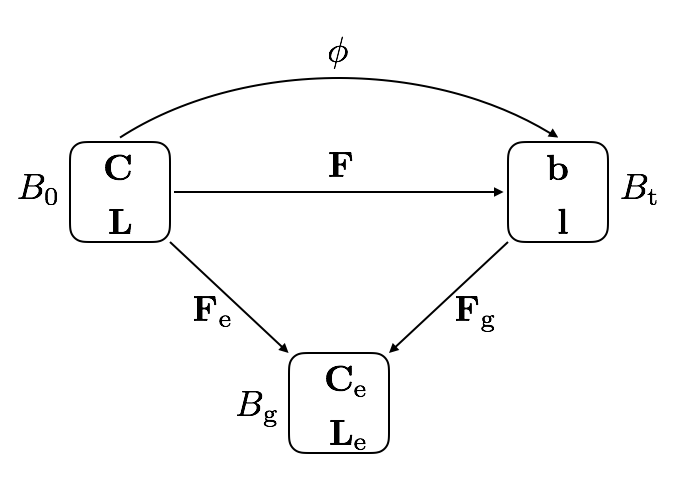
\includegraphics[width=.5\textwidth]{./figures/decomposition.png} % requires the graphicx package
   \caption{The intermediate configuration and the decomposition of deformation gradient}
   \label{fig:decomposition}
\end{figure}

Recall the definition of right Cauchy-Green tensor $\bC$, we define the elastic right Cauchy-Green tensor $\bC_\rme$ analogically as the pull back of the covariant spatial metric $\bold{g}$ to the undeformed reference configuration and to the intermediate configuration, respectively.
\begin{equation} \label{eq:defCe}
\bC = \bF^T \cdot \bg \cdot \bF, \quad \bC_\rme = \bF_\rme^T \cdot \bg \cdot \bF_\rme
=  \bF_\rmg^{-T} \cdot \bC \cdot \bF_\rmg^{-1}
\end{equation}

In Cartesian coordinates, $\bg$ is equal to the identity tensor. The spatial velocity gradient $\bl$, which is defined as the material time derivative of the velocity then can be introduced as:
\begin{equation}
\bl = \nabla_\bx \bv = \dot{\bF} \cdot \bF^{-1}
\end{equation}
The pull back of the spatial velocity gradient to the intermediate configuration
\begin{equation}
\bF_\rme^{-1} \cdot \bl \cdot \bF_\rme = \bL_\rme + \bL_\rmg
\end{equation} 
can be addictively be split into the elastic velocity gradient and the growth velocity gradient:
\begin{equation} \label{eq:L}
\bLe = \bFe^{-1} \cdot \dot{\bFe}, \quad \bLg = \dot{\bFg} \cdot \bFg^{-1} 
\end{equation}
respectively. Figure \ref{fig:configurations} illustrates the kinematics of finite growth in the tangent spaces $TB$ and cotangent spaces $T^*B$ in the reference configuration, the intermediate configuration and the spatial configuration.

\begin{figure}[H]
   \centering
   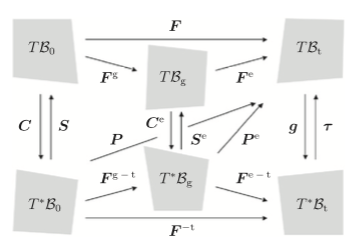
\includegraphics[width=.5\textwidth]{./figures/configurations.png} % requires the graphicx package
   \caption{The kinematics of finite growth}
   \label{fig:configurations}
\end{figure}

Notice the mapping from the reference configuration to the intermediate configuration is "one-to-one", but not "onto", therefore the intermediate configuration is incompatible \cite{Cowin}.

\subsection{Density transformations}
In this section we consider the density expressions in different configurations, which is the basis of the balance equations. Let $\rho_0$ denote the density in the reference configuration, $\rho_\rmt$ and $\rho_\rmg$ denote its counterparts in the spatial configuration and the intermediate configuration, respectively. Similarly, define the volume of a material particle in the reference,  spatial and intermediate configurations as $dV$, $dv$ and $dV_\rmg$, respectively.

In analogy to $J = \mathrm{det}\bF$, define the Jacobians $J_\rme = \mathrm{det}\bFe$ and $J_\rmg = \mathrm{det}\bFg$. The transformations of the volumes become:
\begin{equation} \label{eq:volume}
dv = JdV, \quad dV_\rmg = J_\rmg dV, \quad dv = J_\rme dV_\rmg
\end{equation}
and
\begin{equation} \label{eq:det}
J = J_\rme J_\rmg
\end{equation}

Denote the mass of a material particle as $dM$ and $dm$ in the reference and spatial configuration respectively. Let $R_0$ be a mass source per unit volume in the reference configuration and neglecting the mass flux through the particle surface, the mass balance during the time interval $[t_0, t]$ can be expressed as
\begin{equation} \label{eq:massChange}
dm = dM + \int_{t_0}^t R_0 d\tau dV
\end{equation}
Based on the definitions, we have
\begin{equation} \label{eq:mass}
dm = \rho_\rmg dV_\rmg = \rho_\rmt dv
\end{equation}
Substituting Equation \ref{eq:volume} into Equation \ref{eq:mass}, we obtain the transformation of the density from the spatial configuration to the intermediate configuration:
\begin{equation} \label{eq:density}
\rho_\rmg = J_\rme\rho_\rmt
\end{equation}
Furthermore, define the density of the grown mass in the reference configuration as:
\begin{equation} \label{eq:grown}
\grho = J\rho_\rmt = J_\rmg \rho_\rmg
\end{equation}
The second equivalence is obtained by inserting Equation \ref{eq:det} and \ref{eq:density} into the first one. Substituting Equation \ref{eq:volume}, \ref{eq:mass}, \ref{eq:grown} into \ref{eq:massChange} yields:
\begin{equation} \label{eq:rhoBalance}
\grho = \rho_0 + \int_{t_0}^t R_0 d\tau
\end{equation}
which implies that the density of the grown density equals the initial density and the production of the mass source.

\subsection{Balance laws}
Differentiating Equation \ref{eq:rhoBalance} with respect to time yields the local balance of mass in the reference configuration:
\begin{equation} \label{eq:massBalance}
\dot{\bar{\rho}}_0 = R_0
\end{equation}
Inserting Equation \ref{eq:grown} into \ref{eq:massBalance}, and making use of the identity $\dot{J}_\rmg = J_\rmg \mathrm{tr} \bL_\rmg$ as well as the definition of $\bL_\rmg$ in Equation \ref{eq:L} yields the local balance of mass in the intermediate configuration:
\begin{equation} \label{eq:massBalance2}
\dot{\rho}_\mathrm{g} + \rho_\rmg \mathrm{tr}\bL_\rmg = J_\rmg^{-1}R_0
\end{equation}
In general, the growth in mass can be caused by the increasing of volume (density-preserving), the increasing of density (volume-preserving) or the combination of the both. In this work we assume the growth happens through the increasing of volume as it is common for the soft tissues \cite{Menzel}. In this case the density does not change from the reference configuration to the intermediate configuration. Therefore Equation \ref{eq:massBalance2} becomes:
\begin{equation} \label{eq:massBalance3}
R_0 = J_\rmg\rho_\rmg \mathrm{tr}\bL_\rmg = \grho\mathrm{tr}\bL_\rmg
\end{equation}

The local balance of linear momentum and the entropy inequality are as following:
\begin{equation} \label{eq:momentumBalance}
\grho\dot{\bv} = \grho\bold{B}_0 + \mathrm{DIV}(\bF \cdot \bS)
\end{equation}
\begin{equation} \label{eq:entropy}
\grho D= \frac{1}{2}\bS : \dot{\bC} - \grho \dot \Psi  - \theta\grho s_0 \geq 0
\end{equation}
where $\bold{B}_0$ is the body force, $\bS$ is the second Piola-Kirchhoff stress tensor in the reference configuration, $\Psi$ is the free energy per unit mass and $s_0$ is the extra entropy that is necessary to satisfy the second law of thermodynamics. For the details of the balance laws please refer to \cite{Kuhl2, Lubarda2}.





\section{Constitutive equations}
The elastic deformation can be described with the standard continuum mechanics. While an additional model is needed to characterize the growth deformation as the intermediate configuration is incompatible. In this section we consider a specific constitutive model and a growth model. We restrict the constitutive model to be isotropic. However the extension to anisotropic models should not pose any fundamental difficulty as the multiplicative decomposition approach remains the same. For instance \cite{Goktepe2} presents the application on the anisotropic model.

\subsection{Elastic deformation}
We use the compressible Neo-Hookean model in this work. The free energy is:
\begin{equation}
\Psi = \frac{1}{2}\mathrm{ln}^2 J_\rme + \frac{1}{2}\mu \left[ \bC_\rme : \bI - 3 - 2\mathrm{ln} J_\rme \right]
\end{equation}
where $\lambda$ and $\mu$ are material constants. The elastic second Piola-Kirchhoff stress $\bS_\rme$ and the elastic constitutive moduli $\bbC_\rme$ are derived in a standard way as following:
\begin{equation} \label{eq:Se}
\begin{split}
\bS_\rme &= 2\frac{\partial \Psi}{\partial \bC_\rme} \\
	&= 2\bigg[  \bigg( \frac{\lambda}{2} \bigg) \bigg( \frac{2\mathrm{ln}J_\rme}{J_\rme} \bigg)       \bigg( \frac{J_\rme}{2} \bC_\rme^{-1} \bigg) + \frac{\mu}{2} \bigg( \bI - \frac{2}{J_\rme} \frac{J_\rme}{2} \bC_\rme^{-1} \bigg) \bigg] \\
	&= \left[ \lambda \mathrm{ln}J_\rme - \mu\right]\bC_\rme^{-1} + \mu\bI
\end{split}
\end{equation}
where the identity ${\partial J_\rme}/{\partial \bC_\rme} = J_\rme \bC_\rme^{-1}/2$ is used.
\begin{equation} \label{eq:Ce}
\begin{split}
\bbC_\rme &= 2\frac{\partial \bS_\rme}{\partial \bC_\rme} \\
	&= 2\bigg[ (\lambda \mathrm{ln}J_\rme - \mu) \frac{\partial \bC_\rme^{-1}}{\partial \bC_\rme} + \bC_\rme \otimes \frac{\partial (\lambda \mathrm{ln}J_\rme - \mu)}{\partial \bC_\rme}\bigg] \\
	&= 2\bigg[ (\mu - \lambda \mathrm{ln}J_\rme) \frac{1}{2}(\bC_\rme^{-1} \overline\otimes \bC_\rme^{-1} + \bC_\rme^{-1} \underline\otimes \bC_\rme^{-1}) + \bC_\rme^{-1} \otimes \bigg( \frac{\lambda}{J_\rme}\frac{J_\rme}{2} \bC_\rme^{-1} \bigg) \bigg] \\
	&= (\mu - \lambda \mathrm{ln}J_\rme) (\bC_\rme^{-1} \overline\otimes \bC_\rme^{-1} + \bC_\rme^{-1} \underline\otimes \bC_\rme^{-1} ) + \lambda \bC_\rme^{-1} \otimes \bC_\rme^{-1}
\end{split}
\end{equation}
Note that the equation $\partial\bC_\rme^{-1}/\partial\bC_\rme = -\frac{1}{2}(\bC_\rme^{-1} \overline\otimes \bC_\rme^{-1} + \bC_\rme^{-1} \underline\otimes \bC_\rme^{-1})$ is used, where the operation $\overline\otimes$ and $\underline\otimes$ between two second order tensors $\bA$ and $\bB$ are defined as $(\bA\overline\otimes\bB)_{ijkl} = {\bA}_{ik}{\bB}_{jl}$ and $(\bA\underline\otimes\bB)_{ijkl} = {\bA}_{il}{\bB}_{jk}$ respectively. For more details of the mathematics in continuum mechanics, please refer to \cite{Holzapfel}. 

\subsection{Growth deformation}
To characterize the growth deformation, we explicitly define the growth deformation tensor as the product of the identity tensor and a single scalar $\theta_\rmg$, which is identified as the isotropic stretch ratio due to volumetric mass growth.
\begin{equation} \label{eq:Fg}
\bF_\rmg = \theta_\rmg \bI
\end{equation}
It follows that $J_\rmg = \theta_\rmg ^ 3$. Therefore the grown density in Equation \ref{eq:grown} can be transformed into:
\begin{equation}
\grho = \theta_\rmg^3\rho_\rmg = \theta_\rmg^3\rho_0
\end{equation}
Notice $\rho_\rmg = \rho_0$ as we assume the density does not change during the growth deformation. Meanwhile, the grown velocity gradient in Equation \ref{eq:L} can be expressed as:
\begin{equation}
\bL_\rmg = \frac{\dot\theta}{\theta_\rmg}\bI
\end{equation}
Substituting Equation \ref{eq:Fg} into \ref{eq:massBalance3}, the mass source can be rewritten as:
\begin{equation} \label{eq:massBalance4}
R_0 = \dot{J}_\rmg \rho_0 = 3\rho_0 \theta_\rmg^2\dot\theta_\rmg
\end{equation}
Once the evolution of the stretch ratio is known, the mass source can be determined. There are different assumptions on the evolution of the stretch ratio. For instance \cite{Lubarda2} assumes the evolution of the stretch ratio is driven by the Piola-Kirchhoff stress $\bS_\rme$, while \cite{Goktepe2} and \cite{Himpel} uses the Mandel stress $\bM_\rme = \bC_\rme \cdot \bS_\rme$.
We use the assumption in \cite{Goktepe2} that the growth process is driven by the Mandel stress and the stretch ratio in a discrete form:
\begin{equation} \label{eq:stretchRatio}
\dot\theta_\rmg = k_\rmg(\theta_\rmg)\phi_\rmg(\bM_\rme)
\end{equation}
The growth process is activated only when the pressure, which is measured by the trace of the Mandel stress exceeds a physiological threshold level $M_\rme^{\mathrm{crit}}$:
\begin{equation} \label{eq:stretchRatio2}
\phi_\rmg = \mathrm{tr}(\bM_\rme) - M_\rme^{\mathrm{crit}} \quad \mathrm{with} \quad \frac{\partial \phi_\rmg}{\partial \theta_\rmg} = -\frac{1}{\theta_\rmg} \left[2\mathrm{tr}(\bM_\rme) + \bC_\rme : \bbC_\rme : \bC_\rme\right]
\end{equation}
Function $k_\rmg$ is used to prevent unbounded growth \cite{Lubarda2}:
\begin{equation} \label{eq:stretchRatio3}
k_\rmg = \frac{1}{\tau}\left( \frac{\theta_\mathrm{max} - \theta_\rmg}{\theta_\mathrm{max} - 1} \right)^\gamma
\quad \mathrm{with} \quad 
\frac{\partial k_\rmg}{\partial \theta_\rmg} = -\frac{\gamma}{\theta_\mathrm{max} - \theta\rmg}k_\rmg
\end{equation}
where $\tau$ and $\gamma$ are material constants.

\subsection{Evaluation of stretch ratio, stress, and constitutive moduli}
With all essential definitions introduced, next we discuss the evaluation of the stretch ratio, stress and constitutive moduli. To evaluate the stretch from its time derivative, we apply the implicit Euler backward scheme:
\begin{equation} \label{eq:Euler}
\dot\theta_\rmg = (\theta_\rmg - \theta_\rmg^n)/\Delta t
\end{equation}
and evaluate the residual as:
\begin{equation} \label{eq:residual}
R = \theta_\rmg - \theta_\rmg^\mathrm{n} - \frac{1}{\tau}\left( \frac{\theta_\mathrm{max} - \theta_\rmg}{\theta_\mathrm{max} - 1} \right)^\gamma\left(\mathrm{tr}(\bM_\rme) - M_\rme^{\mathrm{crit}}\right)\Delta t
\end{equation}
To minimize the residual $R$, we linearize Equation \ref{eq:residual} for the tangent moduli $K$:
\begin{equation} \label{eq:K}
K = \frac{\partial R}{\partial \theta_\rmg} =  1 - \left( k_\rmg \frac{\partial \phi_\rmg}{\partial \theta_\rmg} + \phi_\rmg \frac{\partial k_\rmg}{\partial \theta_\rmg} \right)\Delta t
\end{equation}
In the local Newton iteration, where the deformation tensor $\bF$ is known, update the stretch ratio $\theta_\rmg$ with $\theta_\rmg \leftarrow \theta_\rmg - R/K$. The corresponding growth part of the deformation tensor $\bF_\rmg$ can be calculated with Equation \ref{eq:Fg}. Consequently the elastic part $\bF_\rme$ can be calculated with Equation \ref{eq:decomposition}. Then the elastic stress $\bS_\rme$ and elastic constitutive moduli $\bbC_\rme$ can be obtained with Equation \ref{eq:Se} and \ref{eq:Ce} respectively.

As the last step, we need to evaluate the overall stress and constitutive moduli based on the elastic part so that the deformation tensor $\bF$ can be incremented and thus a closed loop can be formed. The second Piola-Kirchhoff stress $\bS$, which will be inserted to the momentum balance equation \ref{eq:momentumBalance} is evaluated as:
\begin{equation}
\begin{split}
\bS &= 2\frac{\partial \Psi}{\partial \bC} \\
	&= 2\frac{\partial \Psi}{\partial \bC_\rme} : \frac{\partial \bC_\rme}{\partial \bC}  \\
	&= 2\frac{\partial \Psi}{\partial \bC_\rme} : \frac{\partial(\bF_\rmg^{-T} \bC \bF_\rmg^{-1})}
	{\partial \bC} \\
	&=  \bF_\rmg^{-1} \cdot 2\frac{\partial \Psi}{\partial \bC_\rme} \cdot \bF_{\rmg}^{-T} \\
	&= \bF_\rmg^{-1} \cdot \bS_\rme \cdot \bF_\rmg^{-T}
\end{split}
\end{equation}
When $\bF_\rmg = \theta_\rmg \bI$, it becomes:
\begin{equation} \label{eq:S}
\bS = \frac{1}{\theta_\rmg^{2}} \bS_\rme
\end{equation}
Its linearization with respect to the total right Cauchy-Green tensor, $\bbC$, which is used in the global Newton iteration, is evaluated with:
\begin{equation} \label{eq:C}
\begin{split}
\bbC &= 2\frac{d\bS(\bF, \bF_\rmg)}{d\bC} \\
	&= 2\frac{\partial\bS(\bF, \bF_\rmg)}{\partial\bC}\bigg|_{\bF_\rmg} + 2\bigg[ \frac{\partial\bS}{\partial\bF_\rmg} : \frac{\partial\bF_\rmg}{\partial\theta_\rmg} \bigg]\otimes \frac{\partial\theta_\rmg}{\partial\bC}\bigg|_{\bF}
\end{split}
\end{equation}
The first term in Equation \ref{eq:C} is the pull back of the elastic moduli $\bbC_\rme$ onto the reference configuration:
\begin{equation} \label{eq:part1}
2\frac{\partial\bS(\bF, \bF_\rmg)}{\partial\bC}\bigg|_{\bF_\rmg} = 2\frac{\partial (\bF_\rmg^{-1} \cdot \bS_\rme \cdot \bF_\rmg^{-T})}{\partial \bC} = (\bF_\rmg^{-1} \overline\otimes \bF_\rmg^{-1}) : \bbC_\rme : (\bF_\rmg^{-T} \overline\otimes \bF_\rmg^{-T})
\end{equation}
Recall the assumption on the growth deformation tensor $\bF_\rmg$ in Equation \ref{eq:Fg}, Equation \ref{eq:part1} is rewritten as:
\begin{equation} \label{eq:term1}
2\frac{\partial\bS(\bF, \bF_\rmg)}{\partial\bC}\bigg|_{\bF_\rmg} = \frac{1}{\theta_\rmg^4}\bbC_\rme
\end{equation}
From Equation \ref{eq:defCe} the elastic right Cauchy-Green tensor $\bC_\rme$ is specified as $\bC_\rme = \bC/\theta_\rmg^2$. Therefore its derivative with respect to the stretch ratio $\theta_\rmg$ is obtained:
\begin{equation} \label{eq:derivativeCe}
\frac{\partial\bC_\rme}{\partial\theta_\rmg} = -\frac{2}{\theta_\rmg^3}\bC = -\frac{2}{\theta_\rmg}\bC_\rme
\end{equation}
Since the growth deformation tensor $\bF_\rmg$ is a function of the stretch ratio $\theta_\rmg$ solely, the second and third term can be evaluated using Equations \ref{eq:S} and \ref{eq:derivativeCe}:
\begin{equation} \label{eq:term23}
\begin{split}
\frac{\partial\bS}{\partial\bF_\rmg} : \frac{\partial\bF_\rmg}{\partial\theta_\rmg}\bigg|_\bF &= \bigg[ \frac{\partial\bS}{\partial\theta_\rmg} +  \bigg(\frac{\partial\bS}{\partial\bS_\rme}\bigg)\cdot \bigg(\frac{\partial\bS_\rme}{\partial\bC_\rme} : \frac{\partial\bC_\rme}{\partial\theta_\rmg}\bigg) \bigg] \bigg|_\bF \\ 
	&= -\frac{2}{\theta_\rmg^3}\bS_\rme + \frac{1}{\theta_\rmg^2} \bigg(\frac{1}{2}\bbC_\rme\bigg) : \bigg( -\frac{2}{\theta_\rmg}\bC_\rme \bigg) \\
	&= -\frac{2}{\theta_\rmg^3}\bigg( \bS_\rme + \frac{1}{2}\bbC_\rme : \bC_\rme \bigg)
\end{split}  
\end{equation}
The fourth term is more complicated. Recall the linearization of the residual of the stretch ratio in Equation \ref{eq:K}, and the assumption of the time derivative of the stretch ratio $\theta_\rmg$ in Equation \ref{eq:Euler}, we have:
\begin{equation}
\theta_\rmg - \theta_\rmg^n =  K\theta_\rmg = k_\rmg\phi_\rmg\Delta t
\end{equation}
The derivative of the stretch ratio $\theta_\rmg$ with respect to the elastic right Cauchy-Green tensor can be expressed as:
\begin{equation} \label{eq:nonsense}
\begin{split}
\frac{\partial\theta_\rmg}{\partial\bC_\rme} &= \frac{k_\rmg}{K} \Delta t \frac{\partial\phi_\rmg}{\partial\bC_\rme}
\end{split}
\end{equation}
where $\partial\phi_\rmg/\partial\bC_\rme$ can be evaluated as:
\begin{equation} \label{eq:derivativePhi}
\frac{\partial\phi_\rmg}{\partial\bC_\rme} = \frac{\mathrm{tr}(\bC_\rme\cdot\bS_\rme)}{\partial\bC_\rme} = \bS_\rme + \frac{1}{2}\bC_\rme : \bbC_\rme
\end{equation}
Substituting Equation \ref{eq:derivativePhi} into Equation \ref{eq:nonsense}, we obtain the fourth term in Equation \ref{eq:C}:
\begin{equation} \label{eq:term4}
\frac{\partial\theta_\rmg}{\partial\bC} = \frac{\partial\theta_\rmg}{\partial\bC_\rme} \frac{\partial\bC_\rme}{\partial\bC} =  \frac{1}{\theta_\rmg^2} \bigg(\frac{k_\rmg}{K}\Delta t\bigg) \bigg( \bS_\rme + \frac{1}{2}\bC_\rme : \bbC_\rme\bigg)
\end{equation}
Putting together Equations \ref{eq:term1}, \ref{eq:term23} and \ref{eq:term4}, Equation \ref{eq:C}, the overall constitutive moduli in total Lagrangian formulation, can be specified as:
\begin{equation} \label{eq:C2}
\bbC = \frac{1}{\theta_\rmg^4}\bbC_\rme - \frac{4}{\theta_\rmg^5}\frac{k_\rmg}{K}\Delta t\bigg(\bS_\rme + \frac{1}{2}\bbC_\rme : \bC_\rme \bigg) \otimes \bigg( \frac{1}{2} \bC_\rme : \bbC_\rme + \bS_\rme \bigg)
\end{equation}
Note that the constitutive moduli $\bbC$ is symmetric.

Pushing forward to the updated Lagrangian formulation is straight-forward. The Kirchhoff stress and the Kirchhoff moduli are:
\begin{equation} \label{eq:tau}
\begin{split}
\boldsymbol{\tau} &= \bF \cdot \bS \cdot \bF^T \\
	&= \theta_\rmg^2 \bF_\rme \cdot \bS \cdot \bF_\rme^T \\
	&= \bF_\rme \cdot \bS_\rme \cdot \bF_\rme^T \\
	&= (\lambda\mathrm{ln}J_\rme - \mu)\bI + \mu\bB_\rme
\end{split}
\end{equation}
and
\begin{equation} \label{eq:tauModuli}
\begin{split}
\bbc &= (\bF \overline\otimes \bF) : \bbC : (\bF^T \overline\otimes \bF^T) \\
	&= \theta_\rmg^4 (\bF_\rme \overline\otimes \bF_\rme) : \bbC : (\bF_\rme^T \overline\otimes \bF_\rme^T) \\
	&= (\bF_\rme \overline\otimes \bF_\rme) : \bbC_\rme : (\bF_\rme^T \overline\otimes \bF_\rme^T) \\
	&+ \frac{4}{\theta_\rmg}\frac{k_\rmg}{K}\Delta t (\bF_\rme \overline\otimes \bF_\rme) :  
	\bigg[(\bS_\rme + \frac{1}{2}\bbC_\rme : \bC_\rme ) \otimes ( \frac{1}{2} \bC_\rme : \bbC_\rme + \bS_\rme )\bigg]
: (\bF_\rme^T \overline\otimes \bF_\rme^T) \\
	&= (\mu - \lambda\mathrm{ln}J_\rme)(\delta_{ik}\delta_{jl} + \delta_{il}\delta_{jk}) + \lambda\delta_{ij}\delta_{kl} \\ 
	&+  \frac{4}{\theta_\rmg}\frac{k_\rmg}{K}\Delta t (\bF_\rme \overline\otimes \bF_\rme) :  
	\bigg[(\bS_\rme + \frac{1}{2}\bbC_\rme : \bC_\rme ) \otimes ( \frac{1}{2} \bC_\rme : \bbC_\rme + \bS_\rme )\bigg]: (\bF_\rme^T \overline\otimes \bF_\rme^T) 
\end{split}
\end{equation}

\subsection{Implementation}
Growth model can be easily implemented within the existing nonlinear finite element framework. In this research the updated Lagrangian formulation is used. Except for the modifications to the Kirchhoff stress and the corresponding constitutive moduli, all the additional computational work it introduces is the iterative solution of the stretch ratio $\theta_\rmg$. Algorithm \ref{algo} lists the major part of the algorithm.

\begin{algorithm}
	\caption{Algorithm for the growth model}  \label{algo}
	\begin{algorithmic}[1]
	\State Given $\bF$ and $\theta_\rmg^n$
	\State $\theta_\rmg \leftarrow \theta_\rmg^n$
	\While{$R > tol$}
	\State compute the elastic tensor $\bF_\rme = \bF/\theta_\rmg$
	\State compute the elastic right Cauchy-Green tensor $\bC_\rme = \bF_\rme^T\cdot\bF_\rme$
	\State compute the elastic second Piola-Kirchhoff stress $\bS_\rme$ using Equation \ref{eq:Se}
	\State compute the growth function $k_\rmg$ using Equation \ref{eq:stretchRatio3}
	\State compute the residual $R$ using Equation \ref{eq:residual}
	\State compute the tangent moduli $K$ using Equation \ref{eq:K}
	\State update stretch ratio $\theta_\rmg \leftarrow \theta_\rmg - R/K$
	\EndWhile
	\State compute the second Piola-Kirchhoff stress $\bS$ using Equation \ref{eq:S}
	\State compute the Kirchhoff stress $\boldsymbol\tau$ using Equation \ref{eq:tau}
	\State compute the Lagrangian moduli $\bbC$ using Equation \ref{eq:Ce}
	\State compute the Kirchhoff moduli $\bbc$ using Equation \ref{eq:tauModuli}
	\end{algorithmic}
\end{algorithm}





\section{Fluid-solid interaction}
Immersed Finite Element Method (IFEM) is a non-boundary-fitted mesh method that represents the background viscous fluid and the immersed deformable solid with different meshes that are independent from each other. The fluid domain $\Omega^\mathrm{f}$ is defined on a fixed Eulerian grid and the solid domain $\Omega^\mathrm{s}$ is constructed independently with a Lagrangian mesh. The fluid exists everywhere in the computational domain and the imaginary fluid in the solid domain is called the ``artificial'' fluid $\bar\Omega$. The interaction between the fluid and the solid is represented by a fluid-solid interaction force $\bold{f}^\mathrm{FSI}$.

The governing equations for the entire computational domain $\Omega$ which includes the real $\Omega^\mathrm{f}$ and the artificial fluid domains $\bar\Omega$, are the Navier-Stokes continuity and momentum equations for incompressible flows:
\begin{subequations} \label{NS}
\begin{align}
\nabla \cdot \bv^\mathrm{f} &= 0 \\
\bar\rho (\bv_{, \mathrm{t}}^\mathrm{f} + \bv^\mathrm{f} \cdot \nabla\bv^\mathrm{f}) &= -\nabla p^\mathrm{f} + \mu\nabla^2 \bv^\mathrm{f} + \bold{f}^\mathrm{FSI,f} + \bar\rho\bold{g} \quad \mathrm{in} \quad \Omega 
\end{align}
\end{subequations}
where  $\bar\rho$ is defined as $\bar\rho = \rho^\mathrm{f} + (\rho^\mathrm{s} - \rho^\mathrm{f})I(\bx)$, while $\rho^\mathrm{f}$ and $\rho^\mathrm{s}$ are the densities of the fluid and the solid, respectively. And the indicator function $I$ is used to identify the artificial fluid from the real fluid. It is set to $1$ in the artificial fluid domain and $0$ in the real fluid domain; and varies from $0$ to $1$ at and near the fluid-structure interface. It needs to be updated as the solid moves or deforms. $\bold{g}$ is the external body force. The $\bold{f}^\mathrm{FSI}$ is defined as the fluid-structure interaction force that represents the viscous effects due to the existence of the solid in the fluid domain. And the superscripts $f$ and $s$ represent fluid and solid variables, respectively. 

The governing equations for the solid, on the other hand, is completely identical to what it would be without fluid, which is introduced in Section \ref{Kinematics}.

Notice the $\bold{f}^\mathrm{FSI}$ is first evaluated in the solid domain $\Omega^\mathrm{s}$ through:
\begin{equation} \label{FSI}
\bold{f}^\mathrm{FSI,s} = \nabla \cdot \boldsymbol{\sigma}^\mathrm{s} - \nabla \cdot \boldsymbol{\sigma}^\mathrm{f} \quad \mathrm{in} \quad \Omega^\mathrm{s}
\end{equation}
where $\boldsymbol\sigma^\mathrm{s}$ is the solid stress evaluated based on the solid constitutive law as a function of the solid deformation; $\boldsymbol\sigma^\mathrm{f}$ is the fluid stress interpolated onto the solid domain from the previous time solution, and then distributed onto the fluid domain as $\Omega^\mathrm{f}$ with the Reproducing Kernel Particle Method (RKPM):
\begin{equation} \label{RKPM}
\bold{f}^\mathrm{FSI,f} = \int_\Omega^\mathrm{s} \bold{f}^\mathrm{FSI,s}\phi(\bx - \bx^\mathrm{s})d\Omega^\mathrm{s}
\end{equation}
where $\phi$ is the interpolation function of the distance of a fluid grid point $\bx$ and a solid point $\bx^s$. Similar procedures also apply to the distribution of the fluid velocity and pressure to the Dirichlet and Neumann boundary conditions of the solid:
\begin{subequations} \label{interpolation}
\begin{align}
q_i &= \left[ v_i^\mathrm{f} \phi(\bx - \bx^\mathrm{s}) \right]\Delta t \quad \mathrm{on} \quad \Gamma^\mathrm{sq} \\
h_i &= \left[ \sigma_{ij}^\mathrm{f} \phi(\bx - \bx^\mathrm{s}) \right]n_j \quad \mathrm{on} \quad \Gamma^\mathrm{sh}
\end{align}
\end{subequations}
Here $q_i$ and $h_i$ are the Dirichlet and Neumann boundary conditions on the solid boundary $\Gamma^\mathrm{sq}$ and $\Gamma^\mathrm{sh}$, respectively. $\Delta t$ is the time step size and $\bold{n}$ is the outward normal of the fluid-structure interface. The numerical algorithm can be described as:
\begin{algorithm}
	\caption{Algorithm for IFEM}  \label{IFEMalgo}
	\begin{algorithmic}[1]
	\State Solve solid equations on the Lagrangian mesh to obtain solid motion and deformation using Algorithm \ref{algo}, using the boundary conditions derived from fluid solutions from the previous time step \label{first}
	\State Compute the fluid-structure interaction force $\bold{f}^\mathrm{FSI}$ using Equation \ref{FSI}
	\State Distribute the fluid-structure interaction force $\bold{f}^\mathrm{FSI}$ onto the fluid domain using Equation \ref{RKPM}
	\State Update the indicator field $I$ based on the relative position of the solid in the fluid domain
	\State Solve fluid equations on the Eulerian mesh to obtain velocity and pressure fields using Equation \ref{NS}
	\State Interpolate fluid velocity and stress onto the solid boundary as its boundary condition using Equations \ref{interpolation} and go back to step \ref{first}
	\end{algorithmic}
\end{algorithm}


\section{Theory of small on large}
Initially proposed by Humphrey in \cite{Baek}, the theory of small on large is an idea to impose a computational process with small characteristic time to a process with large characteristic time. In this method, FSI and the growth are computed alternately with different time steps. To solve the FSI with small time step, the growth is frozen based on the assumption that the growth process is too slow to have a significant effect during a few seconds. Once the FSI computation finishes, an average load of the fluid to the solid tissue could be obtained and used as the external load in the growth simulation, which uses a much larger time step. Notice in the computation of the growth, the change of the external load is neglected since the average load from the previous FSI cycle is used.

Denote the current and next time steps of in the growth model as $t_\mathrm{n}$ and $t_\mathrm{n+1}$. Take a long, straight vessel as an example, the process of the theory of small on large can be illustrated as Figure \ref{fig:smallOnLarge}:
\begin{figure}[H]
   \centering
   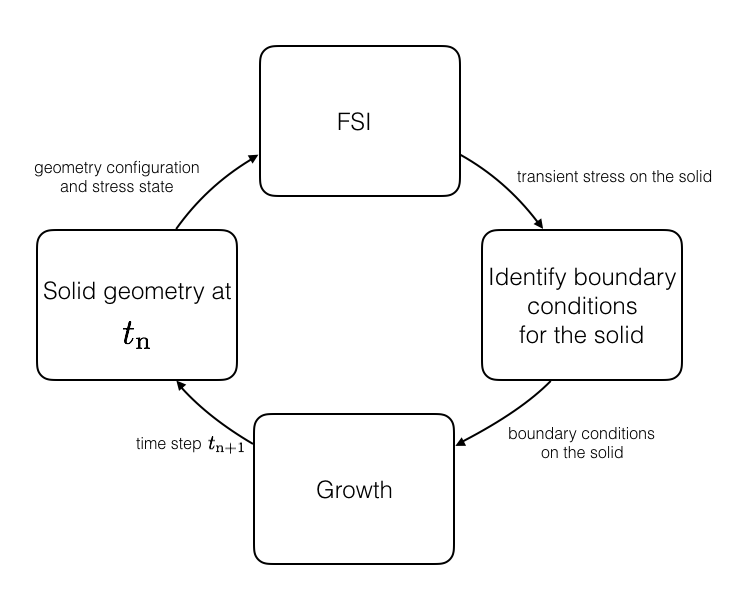
\includegraphics[width=.6\textwidth]{./figures/smallOnLarge.png} % requires the graphicx package
   \caption{Iteration and the information passing in the theory of small on large}
   \label{fig:smallOnLarge}
\end{figure}

The effect of the fluid on the solid is classified as the hydrostatic pressure $p(\bX)$ and wall shear stress $\tau(\bx)$ which are functions of the undeformed coordinates $\bX$. Let $T$ be the computational period of the FSI process, the average pressure $\bar{p}(\bX)$ and wall shear stress $\bar{\boldsymbol{\tau}}(\bX)$ can be obtained as:
\begin{subequations}
\begin{align}
\bar{p}(\bX) &= \frac{1}{T}\int_0^T p(\bX) dt\\
\bar{\boldsymbol{\tau}}(\bX) &= \frac{1}{T}\int_0^T \boldsymbol{\tau}(\bX) dt
\end{align}
\end{subequations}

In \cite{Figueroa}, the theory of small on large was applied with the theory of mixtures which models the arterial wall as a constrained mixture of amorphous elastin matrix, collagen fibers and smooth muscle. In this constrained mixture theory, the growth seeks to maintain a homeostatic biomechanical state via reorganizing and replacing existing constituents with new constituents that have different orientations or mass fractions but identical mechanical properties. In general, the mixture theory may overlook phenomena that can play important biological roles and the role of osmotic pressure \cite{Ambrosi}. Furthermore, although the mixture theory is a self-consistent system, it depends on multiple empirical parameters and is difficult to be combined into finite element framework. Theses factors significantly hinder the application of the mixture theory. The multiplicative growth model used in our research, however, is much more flexible. Not only it allows for different ways to control the growth, but also it can be easily implemented in the existing finite element framework. Combining the theory of small on large with the multiplicative growth model allows us to account for the fluid-structure interaction during the biological growth without the disadvantages of the original content of mixture theory.

\clearpage
\bibliographystyle{plain}
\bibliography{references}

\end{document}  